\section{Implementation}
\label{sec:implementation}

\subsection{Overview}

To meet the performance requirements of the data center, we implemented \OurSys
on the Xilinx Zynq UltraScale+ MPSoC ZCU102 Evaluation Kit.  This platform is
powered by a system-on-chip consisting of a quad-core ARM Cortex-A53, a
dual-core ARM Cortex-R5, and a programmable fabric with 274K lookup tables
(LUTs).
% I guess we need to introduce FPGA more for a network audience...
% Why did we choose to implement on FPGA?
%   Support by example of network paper that performs well on FPGA?

\begin{figure}
  \centering
  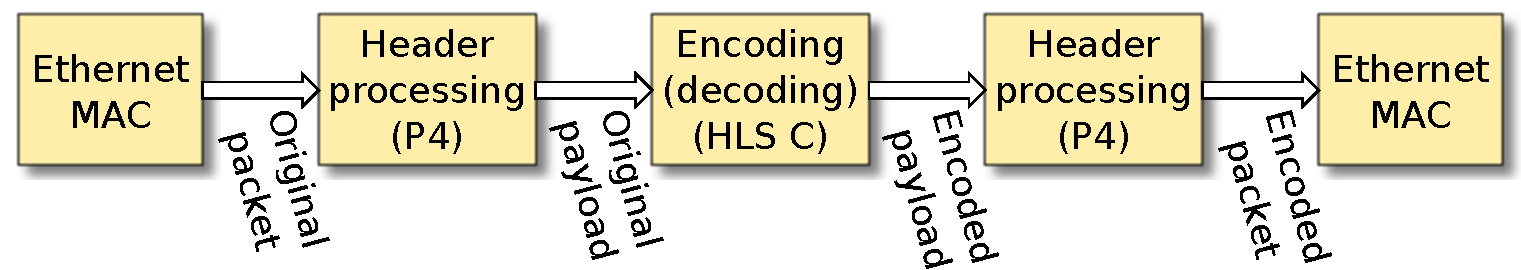
\includegraphics[width=0.4\paperwidth]{Top_level.pdf}
  \caption{\label{fig:toplevel} Block diagram of encoder / decoder pipeline}
\end{figure}

A top-level diagram of the implementation is shown in Fig.~\ref{fig:toplevel}.
Packets arrive on one of the 4 SFP+ cages via a 10Gbps Ethernet cable.
A dedicated Gigabit Transceiver deserializes the packets.  After further
processing by a dedicated Ethernet PHY and in-fabric MAC layer, the entire
packet including Ethernet header is output on a 64-bit AXI Stream bus.

The next stage in the pipeline performs packet header preprocessing.  With
ease of implementation and portability in mind, we implemented this in P4, a
domain-specific programming language for packet processing that is target- and
protocol-agnostic.  The raw payload, i.e. the frame stripped of Ethernet
header, is forwarded to the FEC core.

The FEC core can be an encoder or decoder.  In both cases, the FEC core
produces payloads that are the result of, respectively, encoding or decoding
the received group of payloads.  Similar to the header processing, the FEC core
was also created with ease of implementation in mind.  P4 is not suitable for
exploiting the parallellism of the FEC core, so we described the core in
hardware-synthesizable C.  As usual, the code can be compiled and executed on a
general-purpose CPU.  More importantly, we can synthesize the code for an FPGA
in Vivado HLS.  Guided by pragmas added by the developer, Vivado HLS takes
advantage of parallelism in the code to achieve a high performance.

The encoded or decoded output of the FEC core feeds into the header
post-processing, which encapsulates the payloads in Ethernet packets.  The
Ethernet subsystem, finally, returns the packets to the network.

\subsection{Header processing}

\subsection{FEC encoder}

The current implementation is limited to packet encoding, but our intention is
to implement the decoder too.

Error correction is performed with a Reed-Solomon erasure (RSE) code.  Erasure codes
require prior knowledge of which packets data is missing, as opposed to regular
error correction codes.  This comes with the benefit of requiring fewer error
correction bits.  RSE is a linear code, which means...

\begin{comment}
Introduce P4.
- Advantages of writing in high-level languages.
- Responsibilities of P4.
- Communication between P4 and encoder
Implementation process
- SDNet
- Vivado HLS
- Vivado
Introduce FPGA.
Top-level design
Matrix multiplication
\end{comment}

